%\documentclass[10pt]{beamer} % aspect ratio 4:3, 128 mm by 96 mm
\documentclass[10pt,aspectratio=169]{beamer} % aspect ratio 16:9

%\graphicspath{{../../figures/}}
\graphicspath{{figs/}{../../figures/}{../../../reports/figures/png/}}
%\includeonlyframes{frame1,frame2,frame3,frame4,frame5,frame6,frame7,frame8,frame9}
%\includeonlyframes{frame10,frame11,frame12,frame13}
%\includeonlyframes{frame14,frame15,frame16,frame17,frame18,frame19,frame20,frame21}
%\includeonlyframes{frame22,frame23,frame24,frame25,frame26}
%\includeonlyframes{frame27,frame28}
%%%%%%%%%%%%%%%%%%%%%%%%%%%%%%%%%%%%%%%%%%%%%%%%%%
% Packages
%%%%%%%%%%%%%%%%%%%%%%%%%%%%%%%%%%%%%%%%%%%%%%%%%%
\usepackage{appendixnumberbeamer}
\usepackage{booktabs}
\usepackage{pgfplots}
\usepackage{xspace}
\usepackage{amsmath}
\usepackage{multirow}
\usepackage{totcount}
\usepackage{tikz}
%\usepackage{comment}
%\usetikzlibrary{external} % speedup compilation
%\tikzexternalize % activate!
%\usetikzlibrary{shapes,arrows}  

%\usepackage{bibentry}
%\nobibliography*
\usepackage{caption}%
\captionsetup[figure]{labelformat=empty}%
%%%%%%%%%%%%%%%%%%%%%%%%%%%%%%%%%%%%%%%%%%%%%%%%%%
% Metropolis theme custom modification file
%%%%%%%%%%%%%%%%%%%%%%%%%%%%%%%%%%%%%%%%%%%%%%%%%%
% Metropolis theme custom modification file
%%%%%%%%%%%%%%%%%%%%%%%%%%%%%%%%%%%%%%%%%%%%%%%%%%
% Metropolis theme custom colors
%%%%%%%%%%%%%%%%%%%%%%%%%%%%%%%%%%%%%%%%%%%%%%%%%%
\usetheme[progressbar=foot]{metropolis}
\useoutertheme{metropolis}
\useinnertheme{metropolis}
\usefonttheme{metropolis}
\setbeamercolor{background canvas}{bg=white}

%\usecolortheme{spruce}

\definecolor{myblue}{rgb}{0.19,0.55,0.91}
\definecolor{mediumblue}{rgb}{0,0,205}
\definecolor{darkblue}{rgb}{0,0,139}
\definecolor{Dodgerblue}{HTML}{1E90FF}
\definecolor{Navy}{HTML}{000080} % {rgb}{0,0,128}
\definecolor{Aliceblue}{HTML}{F0F8FF}
\definecolor{Lightskyblue}{HTML}{87CEFA}
\definecolor{logoblue}{RGB}{1,67,140}
\definecolor{Purple}{HTML}{911146}
\definecolor{Orange}{HTML}{CF4A30}

\setbeamercolor{progress bar}{bg=Lightskyblue}
\setbeamercolor{progress bar}{ fg=logoblue} 
\setbeamercolor{frametitle}{bg=logoblue}
\setbeamercolor{title separator}{fg=logoblue}
\setbeamercolor{block title}{bg=Lightskyblue!30,fg=black}
\setbeamercolor{block body}{bg=Lightskyblue!15,fg=black}
\setbeamercolor{alerted text}{fg=Purple}
%%%%%%%%%%%%%%%%%%%%%%%%%%%%%%%%%%%%%%%%%%%%%%%%%%
%  Theme modifications
%%%%%%%%%%%%%%%%%%%%%%%%%%%%%%%%%%%%%%%%%%%%%%%%%%
% modify progress bar linewidth
\makeatletter
\setlength{\metropolis@progressinheadfoot@linewidth}{2pt} 
\setlength{\metropolis@titleseparator@linewidth}{1pt}
\setlength{\metropolis@progressonsectionpage@linewidth}{1pt}

\setbeamertemplate{progress bar in section page}{
	\setlength{\metropolis@progressonsectionpage}{%
		\textwidth * \ratio{\thesection pt}{\totvalue{totalsection} pt}%
	}%
	\begin{tikzpicture}
	\fill[bg] (0,0) rectangle (\textwidth, \metropolis@progressonsectionpage@linewidth);
	\fill[fg] (0,0) rectangle (\metropolis@progressonsectionpage, \metropolis@progressonsectionpage@linewidth);
	\end{tikzpicture}%
}
\makeatother
\newcounter{totalsection}
\regtotcounter{totalsection}

\AtBeginDocument{%
	\pretocmd{\section}{\refstepcounter{totalsection}}{\typeout{Yes, prepending was successful}}{\typeout{No, prepending was not successful}}%
}%
%%%%%%%%%%%%%%%%%%%%%%%%%%%%%%%%%%%%%%%%%%%%%%%%%%
%  Bibliography mods
%%%%%%%%%%%%%%%%%%%%%%%%%%%%%%%%%%%%%%%%%%%%%%%%%%
\setbeamertemplate{bibliography item}{\insertbiblabel} %% Remove book symbol from references and add number in square brackets
% kill the abominable icon (without number)
%\setbeamertemplate{bibliography item}{}
%\makeatletter
%\renewcommand\@biblabel[1]{#1.} % number only
%\makeatother
% remove line breaks in bibliography
\setbeamertemplate{bibliography entry title}{}
\setbeamertemplate{bibliography entry location}{}
%%%%%%%%%%%%%%%%%%%%%%%%%%%%%%%%%%%%%%%%%%%%%%%%%%
%  Bibliography custom commands
%%%%%%%%%%%%%%%%%%%%%%%%%%%%%%%%%%%%%%%%%%%%%%%%%%
\newcommand{\bibliotitlestyle}[1]{\textbf{#1}\par}

\newif\ifinbiblio
\newcounter{bibkey}
\newenvironment{biblio}[2][long]{%
    %\setbeamertemplate{bibliography item}{\insertbiblabel}
    \setbeamertemplate{bibliography item}{}% without numbers
	\setbeamerfont{bibliography item}{size=\footnotesize}
	\setbeamerfont{bibliography entry author}{size=\footnotesize}
	\setbeamerfont{bibliography entry title}{size=\footnotesize}
	\setbeamerfont{bibliography entry location}{size=\footnotesize}
	\setbeamerfont{bibliography entry note}{size=\footnotesize}
	\ifx!#2!\else%
	\bibliotitlestyle{#2}%
	\fi%
	\begin{thebibliography}{}%
		\inbibliotrue%
		\setbeamertemplate{bibliography entry title}[#1]%
	}{%
		\inbibliofalse%
		\setbeamertemplate{bibliography item}{}%
	\end{thebibliography}%
}

\newcommand{\biblioref}[5][short]{
	\setbeamertemplate{bibliography entry title}[#1]
	\stepcounter{bibkey}%
	\ifinbiblio%
	\bibitem{\thebibkey}%
	#2
	\newblock #4
	\ifx!#5!\else\newblock {\em #5}, #3 \fi%
	\else%
	\begin{biblio}{}
		\bibitem{\thebibkey}
		#2
		\newblock #4
		\ifx!#5!\else\newblock {\em #5}, #3\fi
	\end{biblio}
	\fi
}
%
%\newbibmacro*{hypercite}{%
%	\renewcommand{\@makefntext}[1]{\noindent\normalfont##1}%
%	\footnotetext{%
%		\blxmkbibnote{foot}{%
%			\printtext[labelnumberwidth]{%
%				\printfield{prefixnumber}%
%				\printfield{labelnumber}}%
%			\addspace
%			\fullcite{\thefield{entrykey}}}}}
%
%\DeclareCiteCommand{\hypercite}%
%{\usebibmacro{cite:init}}
%{\usebibmacro{hypercite}}
%{}
%{\usebibmacro{cite:dump}}
%
%% Redefine the \footfullcite command to use the reference number
%\renewcommand{\footfullcite}[1]{\cite{#1}\hypercite{#1}}
%%%%%%%%%%%%%%%%%%%%%%%%%%%%%%%%%%%%%%%%%%%%%%%%%%
% Custom commands
%%%%%%%%%%%%%%%%%%%%%%%%%%%%%%%%%%%%%%%%%%%%%%%%%%
% matrix command 
\newcommand{\matr}[1]{\mathbf{#1}} % bold upright (Elsevier, Springer)
%\newcommand{\matr}[1]{#1}          % pure math version
%\newcommand{\matr}[1]{\bm{#1}}     % ISO complying version
% vector command 
\newcommand{\vect}[1]{\mathbf{#1}} % bold upright (Elsevier, Springer)
% bold symbol
\newcommand{\bs}[1]{\boldsymbol{#1}}
% derivative upright command
\DeclareRobustCommand*{\drv}{\mathop{}\!\mathrm{d}}
\newcommand{\ud}{\mathrm{d}}
% 
\newcommand{\themename}{\textbf{\textsc{metropolis}}\xspace}
%%%%%%%%%%%%%%%%%%%%%%%%%%%%%%%%%%%%%%%%%%%%%%%%%%
%  Title page options
%%%%%%%%%%%%%%%%%%%%%%%%%%%%%%%%%%%%%%%%%%%%%%%%%%
% \date{\today}
\date{}
%%%%%%%%%%%%%%%%%%%%%%%%%%%%%%%%%%%%%%%%%%%%%%%%%%
% option 1
%%%%%%%%%%%%%%%%%%%%%%%%%%%%%%%%%%%%%%%%%%%%%%%%%%
\title{Modelling of sandwich plates and piezoelectric transducers to identify the severity of mechanical damage}

\author{\textbf{Piotr Fiborek, M.Sc. Eng.}, \\
	supervisor: Pawel Kudela, D.Sc. Ph.D. Eng.}

% logo align to Institute 

\institute{Institute of Fluid Flow Machinery\\Polish Academy of Sciences \\ \vspace{-1.5cm}\flushright 
\includegraphics[width=4cm]{logo_eng_40mm.eps}}


%%%%%%%%%%%%%%%%%%%%%%%%%%%%%%%%%%%%%%%%%%%%%%%%%%
\begin{document}
%%%%%%%%%%%%%%%%%%%%%%%%%%%%%%%%%%%%%%%%%%%%%%%%%%
\maketitle
% SLIDES
%%%%%%%%%%%%%%%%%%%%%%%%%%%%%%%%%%%%%%%%%%%%%%%%%%
\begin{frame}[label=frame2]{Table of contents \label{frameone}}
  \setbeamertemplate{section in toc}[sections numbered]
  \tableofcontents[hideallsubsections]

\end{frame}
%%%%%%%%%%%%%%%%%%%%%%%%%%%%%%%%%%%%%%%%%%%%%%%%%%
\section{Introduction}
%%%%%%%%%%%%%%%%%%%%%%%%%%%%%%%%%%%%%%%%%%%%%%%%%%
\begin{frame}[label=frame3]{Aim of the research}

	\begin{block}{Aim}

		Investigation of guided wave (GW) propagation in honeycomb sandwich Panel (HSP) using numerical simulations

	\end{block}
	\begin{alertblock}{Thesis}
		Model-assisted analysis of guided wave propagation is an effective tool for determining the damage severity in honeycomb sandwich composites.
	\end{alertblock}

\end{frame}

	\begin{frame}[label=frame2]{Sandwich Composite Properties}

	\begin{columns}[T]

		\column{0.4\textwidth}

		\begin{block}{Sandwich Composite Structures}

			\begin{itemize}

				\item Multi-layered structure composed of a mid-core and thin skins

				\item High strength-to-density ratio

				\item High acoustic or fire insulation properties

			\end{itemize}

		\end{block}

		\column{0.6\textwidth}

		\begin{figure}

			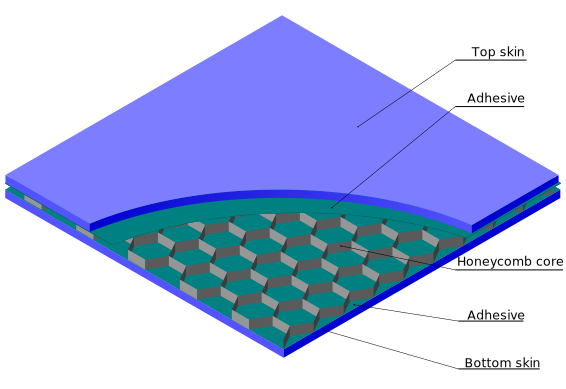
\includegraphics[width=0.75\textwidth]{honeycomb_plate.png}

			\caption{Honeycomb Sandwich Panel (HSP)}

		\end{figure}

	\end{columns}

\end{frame}

\begin{frame}[label=frame6]{Concept of the Method}
\begin{figure}
	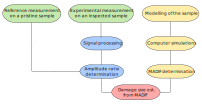
\includegraphics[width=0.9\textwidth]{flowchart.png}
	\caption{A flowchart representing the process for damage size estimation}
\end{figure}
MADIF - Model-assisted Damage Identification Function
\end{frame}


\begin{frame}[label=frame5]{Challenges in modeling of the GW in HSP}
	\footnotesize
	\begin{block}{Challenges}
		\begin{itemize}
			\item complex mesh of the honeycomb core
			\item large number of DOF due to the complexity of the core
			\item large computation time and memory requirements
		\end{itemize}
	\end{block}
	\begin{columns}
		\column{0.5\textwidth}
	\begin{block}{Most common modeling approaches}
		\begin{itemize}
			\item homogenization of the honeycomb core
			\item reduction of the sample dimensions
			\item lack of the adhesive layers
			\item lack of the transducers
		\end{itemize}
	\end{block}
	\column{0.5\textwidth}
	\begin{block}{Present modeling approach}
	\begin{itemize}
		\item application of fast-convergence numerical methods
		\item parallel computation on the GPU
		\item consideration of the adhesive layer
		\item consideration of the PZT transducers
	\end{itemize}
	\end{block}
	\end{columns}
\end{frame}
%%%%%%%%%%%%%%%%%%%%%%%%%%%%%%%%%%%%%%%%%%%%%%%%%%
\section{Development of the Honeycomb Sandwich Panel (HSP) model}
%%%%%%%%%%%%%%%%%%%%%%%%%%%%%%%%%%%%%%%%%%%%%%%%%%
\begin{frame}[label=frame7]{HSP sample configuration}
\begin{table}
	\centering \scriptsize
	\caption{Geometry of HSP [mm]}
	%\begin{tabular}{@{}ccccccc@{}} % remove spaces from vertical lines
	\begin{tabular}{ccccccccccccc} 
		%\hline
		\toprule
		\multicolumn{3}{c}{\textbf{skin}} & {\textbf{adhesive}} & \multicolumn{6}{c}{\textbf{core}} & \multicolumn{2}{c}{\textbf{pzt}} & {\textbf{glue}}\\
		\multicolumn{3}{c}{CFRP $[0^\circ,90^\circ]_s$} & {EA3479B} & \multicolumn{6}{c}{aluminium} & \multicolumn{2}{c}{NCE51} & {CA}\\ 
		%	\hline \hline
		\cmidrule(lr){1-3} \cmidrule(lr){4-4} \cmidrule(lr){5-10} \cmidrule(lr){11-12} \cmidrule(lr){13-13}
		L & W & $g_s$ & $g_a$ & $h_1$ & $h_2$ & $l_1$ & $l_2$ & $g_c$ & $w_c$ & $\Phi$ & $g_t$ & $g_g$\\ 
		%\hline
		%\midrule
		\cmidrule(lr){1-3} \cmidrule(lr){4-4} \cmidrule(lr){5-10} \cmidrule(lr){11-12} \cmidrule(lr){13-13}
		500 & 500 & 1.5 & 0.05 & 11 & 5 & 10.4 & 6 & 14.5 & 0.1 & 10 & 0.5 & 0.05\\
		%\hline 
		\bottomrule 
	\end{tabular} 
	\label{tab:panel_geo}
\end{table}
	\begin{figure}
	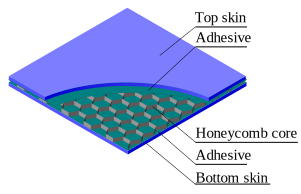
\includegraphics[width=0.75\textwidth]{honeycomb.png}
	\caption{(\textbf{a}) top view of HSP, (\textbf{b}) panel components, (\textbf{c}) details of the honeycomb cell}
	\end{figure}
\note{The object of our research is a sample consisting of carbon skin bonded to aluminium honeycomb.The panel is open on one side so that there is an opportunity to increase the damage. The cell core is a irregular hexagonal with double thickness, from technological point of view, vertical walls.}
\end{frame}

%%%%%%%%%%%%%%%%%%%%%%%%%%%%%%%%%%%%%%%%%%%%%%%%%%
\begin{frame}[label=frame8]{Basis of the Spectral Element Method}
	\begin{itemize}
		\item Division of the domain into non-overlapping spectral elements
		\item Nodes distribution - endpoints of the element and roots of the first derivative of Legendre polynomial \(\mathcal{P}\) of degree \(p\):
		\textcolor{red}{wstawic obrzek elementu z wezlami}
		\begin{equation*}
			(1-\xi^2)\mathcal{P}'_{p}(\xi)=0.
			\label{eq:nodes}
		\end{equation*}
		\item Gauss-Lobatto-Legrendre (GLL) integration scheme:
		\begin{equation*}
			{w(\xi)} = \frac{2}{p(p+1)(\mathcal{P}_{p}(\xi))^2}.
			\label{eq:weight}
		\end{equation*}
		\item Imposing external forces \(f_{ext}\) and boundary conditions
		\item Equation of motion:
		\begin{equation*}
			\label{eq:motion}
			\textbf{M} \ddot{d} + \textbf{D} \dot{d} + \textbf{K} d = f_{ext}
		\end{equation*}
		\item Diagonal mass matrix $\textbf{M}$
	\end{itemize}
\end{frame}

\begin{frame}[label=frame11]{Meshes for the components with the interfaces}
	\begin{figure}
		\includegraphics[width=0.78\linewidth]{panel_mesh.png}
		\caption{The meshes of HSP components and the interfaces}
		\label{fig:panel_mesh}
	\end{figure}
\end{frame}
\begin{frame}[label=frame12]{Disbonds models}
	\
	\begin{figure}
		\includegraphics[width=1\linewidth]{disbond.png}
		\caption{The damaged area in the: (\textbf{a}) experimental sample, (\textbf{b}) numerical model with removed cells and (\textbf{c}) numerical model with interface decoupling}
		\label{fig:disbonds}
	\end{figure}
\end{frame}
\begin{frame}[label=frame11]{Comparison of the models healthy state}
\begin{figure}
	\includegraphics[width=1\linewidth]{figs/fullfield_100_0}
	\label{fig:fulfield_100kHz_0}
\end{figure}
\end{frame}
\begin{frame}[label=frame11]{Comparison of the models - damage 90 mm}
\begin{figure}
	\includegraphics[width=1\linewidth]{figs/fullfield_100_90}
	\label{fig:fulfield_100kHz_90}
\end{figure}
\end{frame}
\section{Experimental Validation of the Method }
%%%%%%%%%%%%%%%%%%%%%%%%%%%%%%%%%%%%%%%%%%%%%%%%%%
\begin{frame}[label=frame13]{Experimental validation setup}
	\begin{columns}[T]
		\column{0.55\textwidth}
	\begin{figure}
		\includegraphics[width=0.7\linewidth]{pzt_setup.png}
		\footnotesize
		\caption{(\textbf{a}) the wave generation/acquisition setup: DMU - the data management unit, G1, G2 - the arbitrary wave generator, O - the oscilloscope, HVA - the voltage amplifier, LWDS - the Lamb Wave Detection Systems, (\textbf{b}) the specimen with PZTs}
		\label{fig:pzt_setup}
	\end{figure}
		\column{0.45\textwidth}
		\begin{figure}
			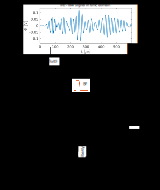
\includegraphics[width=0.8\linewidth]{signal_processing.png}
			\caption{Flowchart for signal processing}
			\label{fig:signal_processing}
		\end{figure}
	\end{columns}	
\end{frame}
\begin{frame}[label=frame14]{Experimental validation results - single skin plate}
		\begin{figure}
			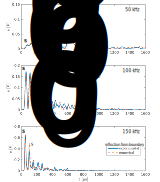
\includegraphics[width=1\linewidth]{single_skin.png}
			\label{fig:single_skin}
		\end{figure}
\end{frame}

\begin{frame}[label=frame15]{Experimental validation results - single CFRP}
	\begin{table}
		\centering
		\caption{\label{tab:group_velocity_cfrp} Comparison between amplitudes and group velocities obtained from the simulations and experiments for single skin plate}
		\begin{tabular}{cccccccc}
			\toprule
			& & \multicolumn{3}{c}{\(C_g\)} & \multicolumn{3}{c}{Amp.}\\
			Mode & Frequency & Exp. & Num. & \(\delta\)& Exp. & Num. & \(\delta\)\\
			& kHz & m/s & m/s & \% & mV & mV & \% \\
			\midrule
			\multirow{3}{*}{$S_0$} & 50 & 6079 & 5865 & \textcolor{green}{3.52}& 12 & 15 & \textcolor{red}{25.0} \\
			&100& 5571 & 5747 & \textcolor{green}{3.16} & 15 & 162 & \textcolor{green}{5.26}\\
			&150& 5764 & 5698 & \textcolor{green}{1.15} & 648 & 664 & \textcolor{green}{2.47}\\
			\midrule
			\multirow{3}{*}{$A_0$} &50& 1341 & 1325 & \textcolor{green}{0.74} & 134 & 125 & \textcolor{green}{6.72}\\
			&100& 1550 & 1396 & \textcolor{green}{9.74} & 84 & 104 & \textcolor{red}{23.8}\\
			\bottomrule
		\end{tabular}
	\end{table}
\end{frame}
\begin{frame}[label=frame15]{Experimental validation results - HSP based on the full core geometry model (\textbf{FCGM}) }
	\begin{figure}
			\includegraphics[width=1\linewidth]{HSP_full.png}
			\label{fig:HSP_full}
		\end{figure}
\end{frame}
\begin{frame}[label=frame16]{Experimental validation results - HSP}
	\begin{table}
		\centering
		\caption{\label{tab:group_velocity_hsp} Comparison between amplitudes and group velocities obtained from the simulations based on the FCGM and experiments for HSP}
		\begin{tabular}{cccccccc}
			\toprule
			& & \multicolumn{3}{c}{\(C_g\)} & \multicolumn{3}{c}{Amp.}\\
			Mode & Freq. & Exp. & FCGM & \(\delta\) & Exp. & FCGM & \(\delta\)\\
			& kHz & m/s & m/s & \% & mV & mV & \%\\
			\midrule
			\multirow{3}{*}{$S_0$} & 50 & 6452 & 8696 & {34.78}& 32 & 6 & \textcolor{red}{81.25}\\
			&100& 5263 & 5128 & \textcolor{green}{2.57}& 369 & 314 & \textcolor{green}{14.91}\\
			&150& 5085 & 5217 & \textcolor{green}{2.60}& 1341 & 1239 & \textcolor{green}{7.61}\\
			\midrule
			\multirow{2}{*}{$A_0$} & 50 & 966 & 926 & \textcolor{green}{4.14} & 1316& 76 & {22.58}\\
			& 100 & 2174 & 2151 & \textcolor{green}{1.06} & 137 & 179 & {30.66}\\
			\bottomrule
		\end{tabular}
	\end{table}
\end{frame}
\section{Model-Assisted Damage Identification Function}
%%%%%%%%%%%%%%%%%%%%%%%%%%%%%%%%%%%%%%%%%%%%%%%%%%
\begin{frame}[label=frame17]{Model-Assisted Damage Identification Function (MADIF)}
\begin{figure}
	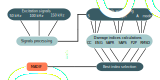
\includegraphics[width=1\linewidth]{madif_extract.png}
	\label{fig:madif_ectract}
\end{figure}
\end{frame}

\begin{frame}[label=frame17]{Damage Idices (DI) - full length signals}
	\begin{figure}
		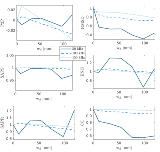
\includegraphics[width=1\linewidth]{DI_full_full.png}
		\label{fig:DI_full_full}
	\end{figure}
\end{frame}
\begin{frame}[label=frame17]{Damage Idices (DI) - S\(_0\) mode}
	\begin{figure}
		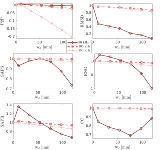
\includegraphics[width=1\linewidth]{DI_full_S0.png}
		\label{fig:DI_full_S0}
	\end{figure}
\end{frame}
\begin{frame}[label=frame17]{Damage Idices (DI) - A\(_0\) mode}
\begin{figure}
	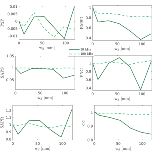
\includegraphics[width=1\linewidth]{DI_full_A0.png}
	\label{fig:DI_full_A0}
\end{figure}
\end{frame}

\begin{frame}[label=frame21]{MADIF determination - full length 100 kHz signal}
		
		\begin{columns}[T]
			\column{0.4\textwidth}
			\begin{block}{MADIF determination}
				\begin{itemize}
					\item Fitting functions:\\
					\footnotesize
					\begin{equation*}
						f_1(x) = \frac{a_2x}{(x+a_1)}+a_0
						\label{eq:f1}
					\end{equation*}
					\begin{equation*}
						f_2(x) = a_2\sqrt{x}+a_1x +a_0
						\label{eq:f2}
					\end{equation*}
					\begin{equation*}
						f_3(x) = \frac{a_3x}{\sqrt{a_2x^2+a_1}}+a_0
						\label{eq:f3}
					\end{equation*}
				\end{itemize}
					\begin{itemize}
						\item Mean absolute error:\\
						\footnotesize
						\begin{equation*}
							\delta^{\mathrm{fit}} = \frac{1}{\mathrm{n^{DI}}}\sum_{i=1}^{\mathrm{n^{DI}}} \left|\frac{\mathrm{DI^i_{n}}-f(x^i)}{\mathrm{DI^i_{n}}}\right|\times100
							\label{eq:delta}
						\end{equation*}
					\end{itemize}
				\end{block}
				\column{0.6\textwidth}
				\begin{figure}
					\includegraphics[width=1\linewidth]{RMSD.png}
					\label{fig:RMSD_full_100}
				\end{figure}
			\end{columns}

\end{frame}

\begin{frame}[label=frame22]{MADIF vs. experimental results}
	\begin{block}{MADIF based on RMSD for full length 100 kHz signal with interface removed model}
		\footnotesize
		\begin{equation*}
			\mathrm{MADIF}^\mathrm{RMSD} = \frac{13.44w_d}{(w_d+38.12)}+0.64
			\label{eq:rmsd}
		\end{equation*}
	\end{block}
\begin{figure}
	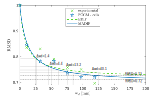
\includegraphics[width=0.8\linewidth]{MADIF_RMSD.png}
	\label{fig:MADIF_RMSD}
\end{figure}
\end{frame}
\begin{frame}[label=frame22]{MADIF vs. experimental results}
	\begin{block}{MADIF based on CC for full length 100 kHz signal with interface removed model}
		\footnotesize
		\begin{equation*}
			\mathrm{MADIF}^\mathrm{CC} = \frac{16.62w_d}{(w_d+133.05)}+0.88
			\label{eq:cc}
		\end{equation*}
	\end{block}
	\begin{figure}
		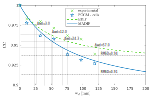
\includegraphics[width=0.8\linewidth]{MADIF_CC.png}
		\label{fig:MADIF_CC}
	\end{figure}
\end{frame}
%%%%%%%%%%%%%%%%%%%%%%%%%%%%%%%%%%%%%%%%%%%%%%%%%%%%%%%%%%%%%%%%%%%%%%%%%%%%%%%%%%
\section{Parametric study}
\begin{frame}[label=frame25]{Parametric study}
	\begin{enumerate}
		\item The effect of ambient temperature on the MADIF:
		\item The PZT parameters:
		\begin{itemize}
			\item placement in relation to the core cell
			\item charge constant
			\item dielectric permittivity.
		\end{itemize}
		\item The CFRP and the adhesive layer parameters:
		\begin{itemize}
			\item CFRP fibre volume fraction
			\item adhesive layer thickness.
		\end{itemize}
		\item The core parameters:
		\begin{itemize}
			\item core height and width
			\item wall thickness
			\item core rotation angle regarding to wave propagation.
		\end{itemize}
	\end{enumerate}
\end{frame}

\begin{frame}[label=frame24]{Temperature-dependent material properties}
	\begin{figure}
		\includegraphics[width=1\linewidth]{skin_temp.png}
		\label{fig:SKIN_TEMP}
	\end{figure}
\end{frame}

\begin{frame}[label=frame24]{Temperature-dependent material properties - PZT}
	\begin{figure}
		\includegraphics[width=1\linewidth]{pzt_temp.png}
		\label{fig:PZT_TEMP}
	\end{figure}
\end{frame}

\begin{frame}[label=frame24]{Effect of ambient temperature on MADIF - RMSD}
	\begin{figure}
		\includegraphics[width=1\linewidth]{MADIF_RMSD_TEMP.png}
		\label{fig:MADIF_RMSD_TEMP}
	\end{figure}
\end{frame}
\begin{frame}[label=frame24]{Effect of ambient temperature on MADIF - CC}
	\begin{figure}
		\includegraphics[width=1\linewidth]{MADIF_CC_TEMP.png}
		\label{fig:MADIF_CC_TEMP}
	\end{figure}
\end{frame}
\begin{frame}[label=frame25]{Effect of the PZT parameters on GW propagation}
	\begin{figure}
		\begin{center}
			\includegraphics[width=0.5\textwidth]{pzt_place}
		\end{center}
		\caption{The GW propagation in the HSP (\textbf{a}), sensor responses for (\textbf{b}) different PZT placement in relation to the core cell}
		\label{fig:pzt_place}
	\end{figure}
\end{frame}

\begin{frame}[label=frame25]{Effect of the PZT parameters on GW propagation}
	\begin{figure}
		\begin{center}
			\includegraphics[width=0.8\textwidth]{pzt_eps}
		\end{center}
		\caption{The signal envelopes for \textbf{the piezoelectric dielectric permittivity} in the range of 80\%-120\% of the reference value}
		\label{fig:pzt_eps}
	\end{figure}
\end{frame}
\begin{frame}[label=frame25]{Effect of the adhesive thickness on GW propagation}
	\begin{figure}
		\begin{center}
			\includegraphics[width=0.8\textwidth]{adhesive_thickness}
		\end{center}
		\caption{The signal envelopes for the various \textbf{adhesive thickness} in the range 100-500 \(\mu\)m}
		\label{fig:adhesive_thickness}
	\end{figure}
\end{frame}
\begin{frame}[label=frame25]{Effect of the reinforcing fibres volume fraction on GW propagation}
	\begin{figure}
		\begin{center}
			\includegraphics[width=0.8\textwidth]{skin_volume}
		\end{center}
		\caption{The signal envelopes for various \textbf{the reinforcing fibres volume fraction} in the range 45-50 \%}
		\label{fig:the reinforcing fibres volume fraction}
	\end{figure}
\end{frame}
\begin{frame}[label=frame25]{Effect of the core parameters on GW propagation}
	\begin{figure}
		\begin{center}
			\includegraphics[width=0.8\textwidth]{core_size}
		\end{center}
		\caption{The signal envelopes for the various \textbf{the core size} in the range 5.0-9.0 mm}
		\label{fig:core_size}
	\end{figure}
\end{frame}

\begin{frame}[label=frame25]{Effect of the core parameters on GW propagation}
	\begin{figure}
		\begin{center}
			\includegraphics[width=0.8\textwidth]{core_height}
		\end{center}
		\caption{The signal envelopes for the various \textbf{core heights} in the range 10.5-18.5 mm}
		\label{fig:core_height}
	\end{figure}
\end{frame}

%%%%%%%%%%%%%%%%%%%%%%%%%%%%%%%%%%%%%%%%%%%%%%%%%%%%%%%%%%%%%%%%%%%%%%%%%%%%%%%%%%%
\section{Final remarks}
\begin{frame}[label=frame24]{Final remarks}
	\begin{alertblock}{Conclusions}
		\begin{itemize}
			\item study proved the validity of the thesis that model-assisted analysis is an effective tool for the determining the damage severity in honeycomb composites
			\item better agreement of the MADIF based on FCGM than HCGM
			\item insufficient accurate model for low temperatures
		\end{itemize}
	\end{alertblock}
\begin{alertblock}{Future works}
	\begin{itemize}
		\item analyzing the functions for damage with different shapes and various localization
		\item develop HSP material properties optimization tool
	\end{itemize}
\end{alertblock}
\end{frame}
{\setbeamercolor{palette primary}{fg=black, bg=white}
	\begin{frame}[standout]
		Thank you for your attention!\\ \vspace{12pt}
		\scriptsize{\url{pfiborek@imp.gda.pl}}
		\begin{block}{Acknowledgement}
			\tiny
			Author would like to gratefully acknowledge the support given by the National Science, Poland under agreement no. 2018/31/N/ST8/02865 in the frame of PRELUDIUM project entitled: 'Model-assisted damage identification function for Structural Health Monitoring of composite structures under a varied environmental condition'
			\begin{figure}
				\includegraphics[width=0.25\linewidth]{NCN.png}
				\label{fig:NCN}
			\end{figure}
		\end{block}
	\end{frame}
}
\end{document}